\chapter{Assertions and Questions}\label{chap:introduction}

\begin{flushright}
	~\hfill 
\includegraphics[width=.18\linewidth]{./images/margol.png}\newline\vspace{5mm}
	Margol, Az Mah
\end{flushright}


Assertions and questions can be seen as the two sides of the same coin, as they form the two core building blocks of any given conversation. Question typically request information, while assertions typically provide information. (\ref{ex1:simple-q}) for instance, is a question that requests information about the country where Jo grew up (presupposing there is one such country). (\ref{ex1:simple-a}) can be seen as a good (assertive) answer to this question, providing the piece of information that Jo grew up in France. Semanticists have observed that the pairs formed by questions and answers are restricted: some are obviously good, while some others are (sometimes surprisingly) odd. So, questions and answers have to be somewhat \textit{congruent}. For instance, (\ref{ex1:simple-bad-a}) cannot be seen as a suitable answer to (\ref{ex1:simple-q}), even if it seems to indicate something about Jo's nationality.

\begin{exe}
	\ex\label{ex1:simple-q-a}
	\begin{xlist}
		\ex[] {In which country did Jo grow up?}\label{ex1:simple-q}
		\ex[] {--Jo grew up in France.}\label{ex1:simple-a}
		\ex[\#] {--Jo speaks French natively.}\label{ex1:simple-bad-a}
	\end{xlist}
\end{exe}

This Chapter motivates and lays the foundation of the main contribution of this dissertation: a constrained machinery ``retro-engineering'' questions out of assertions, allowing to capture intricate patterns in the domain of pragmatic oddness, that were not previously seen as an issue of question-answer congruence. This Chapter is organized as follows. Section \ref{sec:assertions} provides a broad overview of the semantics of assertions, and discusses to what extent they can meaningfully contribute to a conversation. Section \ref{sec:questions} turns to the semantics and pragmatics of questions and highlights how questions relate to alternative assertions, and their possible answers. Section \ref{sec:q-a-interaction} bridges Sections \ref{sec:assertions} and \ref{sec:questions}, by discussing how questions further constrain which assertions should matter in a given conversation. It also points out a few cases in which question-answer is (seemingly) unhelpful. Section \ref{sec:q-derivation} constitutes a more technical appendix sketching how the semantics of questions is standardly derived. This whole Chapter heavily builds on the section of \textcite{Heim2023} dedicated to Questions.


\section{Assertions provide information in the form of propositions}\label{sec:assertions}

\subsection{Extension and intension of assertions}
When studying the semantics of natural language expressions, one usually starts with assertions, because they appear intuitively simpler. We will use the simple assertion in (\ref{ex1:simple-a}), as a running example. At the most basic level, assertions are truth-conditional, i.e. their meaning corresponds to the set of conditions under which they hold. For instance, \textit{Jo grew up in France} will be true if and only if whoever \textit{Jo} is, grew up in whatever geographical entity \textit{France} is. The \textit{extension} of an assertion is therefore of type \texttt{t}, the type of truth-values.

Additionally, the truth-conditions of a sentence are parametrized by (at least) a world variable.\footnote{Other parameters can also be relevant, like times, and assignments. But we choose to keep things simple here.}. So, \textit{Jo grew up in France} will be true as evaluated against a world $w_0$ if and only if whoever \textit{Jo} is in $w_0$, grew up in $w_0$ in whatever geographical entity \textit{France} is in $w_0$. One can then abstract over this world-parameter, and define the \textit{intension} of an assertion as a function from worlds to truth-values. Such functions are called \textit{propositions}, and have type $\langle \texttt{s}, \texttt{t}\rangle$, where \texttt{s} is the type of world-variables. So, the intension, or propositional content of \textit{Jo grew up in France}, will be a function mapping any world variable $w$, to true if and only if, whoever \textit{Jo} is in $w$, grew up in $w$ in whatever geographical entity \textit{France} is in $w$. This is formalized (with some simplifications) in (\ref{ex1:prop-func}).

\begin{exe}
	\ex {$\llbracket$ Jo grew up in France $\rrbracket$ = $\lambda w. \ $ Jo grew up in France in $w$\\
		\phantom{$\llbracket$ Jo grew up in France $\rrbracket$} : $\langle \texttt{s}, \texttt{t}\rangle$}\label{ex1:prop-func}
\end{exe}

Propositions can receive an alternative, equivalent interpretation in terms of sets, based on the idea that any function with domain $D$ and range $R$ is just a (potentially infinite) set of pairs of elements in $D\times R$. A proposition is then simply the set of worlds in which it holds. This interpretation of propositions will be heavily used throughout the dissertation, and is outlined in (\ref{ex1:prop-func-set}). 

\begin{exe}
	\ex {$\llbracket$ Jo grew up in France $\rrbracket$ = $\lambda w. \ $ Jo grew up in France in $w$\\
		\phantom{$\llbracket$ Jo grew up in France $\rrbracket$} $\simeq$ $\lbrace w \ | \ $ Jo grew up in France in $w$ $\rbrace$}\label{ex1:prop-func-set}
\end{exe}

\subsection{Assertions in conversation}
Propositions either denote functions of type $\langle \texttt{s}, \texttt{t}\rangle$, or subsets of the set of elements of type \texttt{s}. Should all elements of type \texttt{s} be considered when evaluating such functions, or computing such subsets? It is commonly assumed that the worlds under consideration at any point of a conversation, are the ones that are compatible with the premises of the said conversation \parencite{Stalnaker1974,Stalnaker1978}. For instance, if two people have a discussion about \textit{France}, it is often reasonable to assume that they agree on what geographical area \textit{France} encompasses, and more generally about the topology of Earth. Moreover, they agree that they agree on this; and agree that they agree that they agree on this; etc. Propositions subject to this recursive, mutual, tacit agreement pattern, form what is called a Common Ground (henceforth \textbf{CG}, \parencite{Stalnaker1978}). Each conversation has its own CG, as defined in (\ref{ex1:common-ground}). The set of worlds in which all the propositions of the CG hold, is called the Context Set (henceforth \textbf{CS}). The CS associated with a conversation is therefore a subset of the set of all possible worlds; and can also be seen (under the set interpretation of propositions) as the grand intersection of the propositions in the CG. This is defined in (\ref{ex1:context-set}).

\begin{exe}
	\ex {\textsc{\textbf{Common Ground (\textbf{CG})}}. Let $\mathcal{C}$ be a conversation between participants $\lbrace P_1, ..., P_k \rbrace$. Let $K(x, p)$ is a proposition meaning that individual $x$ knows $p$, and $p$ is a proposition. The Common Ground of $\mathcal{C}$ is the set of propositions that are recursively taken for granted by all the participants in $\mathcal{C}$:\\
	$p \in CG(\mathcal{C}) \iff \forall n \in \mathbb{N}^*. \ \forall \lbrace k_1, ... k_n \rbrace \in [1; k]^n. \ K(P_{k_1}, K(P_{k_2},...K(P_{k_n}, p)...)$ }\label{ex1:common-ground}
	\ex {\textsc{\textbf{Context Set (\textbf{CS})}}. Let $\mathcal{C}$ be a conversation between participants $\lbrace P_1, ..., P_k \rbrace$. Let CG $CG(\mathcal{C})$ be the Common Ground of this conversation. Under a set interpretation of propositions, the resulting Context Set $CS(\mathcal{C})$ is the set of worlds verifying all propositions of the CG, i.e.:\\
		$CS(\mathcal{C}) = \bigcap\lbrace p \ | \ p \in CG(\mathcal{C})\rbrace$.} \label{ex1:context-set}
\end{exe}


The concepts of CG and CS help delineate which worlds to focus on when evaluating an assertion in context, and determining to what extent this assertion is informative. If uttering an assertion is akin to \textit{adding} it to the CG, then, it also amounts to \textit{intersecting} this assertion with the CS.

\begin{exe}
	\ex {\textsc{\textbf{Updating the Common Ground}}. Let $\mathcal{C}$ be a conversation, and $CG(\mathcal{C})$ its Common Ground. If a sentence $S$ denoting $p$ is uttered, then $p$ is added to $CG(\mathcal{C})$ to form a new Common Ground $CG'(\mathcal{C})$:\\
	$CG'(\mathcal{C}) = CG(\mathcal{C}) \cup \lbrace p\rbrace$}\label{ex1:common-ground-update}
	\ex {\textsc{\textbf{Updating the Context Set}}. Let $\mathcal{C}$ be a conversation and $CS(\mathcal{C})$ its Context Set. If a sentence $S$ denoting $p$ is uttered, then a new Context Set $CS'(\mathcal{C})$ is derived by intersecting $CS(\mathcal{C})$ with $p$:\\
	$CS'(\mathcal{C}) = CS(\mathcal{C}) \cap p$}\label{ex1:context-set-update}
	\ex {\textsc{\textbf{Link between the two updates}}. (\ref{ex1:context-set-update}) can be derived from (\ref{ex1:common-ground-update}) and the definition of the CG in (\ref{ex1:context-set}):\\
		$CS'(\mathcal{C}) = \bigcap\lbrace q \ | \ q \in CG'(\mathcal{C})\rbrace$\\
		\phantom{$CS'(\mathcal{C})$} $= \bigcap\lbrace q \ | \ q \in CG(\mathcal{C}) \cup \lbrace p\rbrace\rbrace$\\
		\phantom{$CS'(\mathcal{C})$} $= \bigcap\lbrace q \ | \ q \in CG(\mathcal{C})\rbrace \cap p$\\
		\phantom{$CS'(\mathcal{C})$} $= CS(\mathcal{C}) \cap p$}
\end{exe}

Note that updating the CG will always create a bigger set, because the CG is simply a collection of propositions. For instance, if \textit{Jo grew up in Paris} is already in the CG, then, adding the proposition denoted by \textit{Jo grew up in France} to the CG will mechanically expand it. Updating the CS however, does not always lead to a different, smaller CS. For instance, taking for granted that Paris is in France (i.e., all the \textit{Paris}-worlds of the CS are \textit{France}-worlds), and assuming that \textit{Jo grew up in Paris} is already common ground, intersecting the CS with the proposition that \textit{Jo lives in France} will not have any effect. This seems to capture the idea that a proposition like \textit{Jo lives in France} is \textit{uninformative} once it is already known by all participants that \textit{Jo lives in Paris}.

More generally, if it is Common Ground that $p$, and a sentence $S$ denoting $p^-$ s.t. $p \vDash p^-$ is uttered, then $S$ will feel uninformative. An informative assertion should lead to a non-vacuous update of the CS, i.e. it should properly \textit{shrink} the CS. This is spelled out in (\ref{ex1:informativity}).

\begin{exe}
	\ex {\textsc{\textbf{Informativity}} (propositional view). A sentence $S$ denoting a proposition $p$ is informative in a conversation $\mathcal{C}$, iff $CS(\mathcal{C}) \cap p \subset CS(\mathcal{C})$.}\label{ex1:informativity}
\end{exe}


In that framework, an assertion provides information in the sense that it reduces the set of live possibilities, and allows to better guess which world is the ``real'' one. Figure \ref{fig1:informative-assertions} illustrates how an asserted proposition can be informative or uninformative, depending on its set-theoretic relationship to the CS.

\begin{figure}[H]
	\centering
	\begin{subfigure}[b]{.23\linewidth}
		\centering
		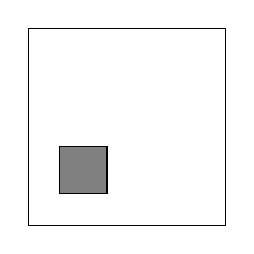
\begin{tikzpicture}	
			\draw [draw=black] (0, 0) rectangle (2.5, 2.5);
			\filldraw [draw=black,fill=gray] (0.4, 0.4) rectangle (1, 1);
		\end{tikzpicture}
		\caption{Informative update ($p$ strictly contained in the CS).}\label{fig1:contained-update}
	\end{subfigure}\hfill
	\begin{subfigure}[b]{.23\linewidth}
		\centering
		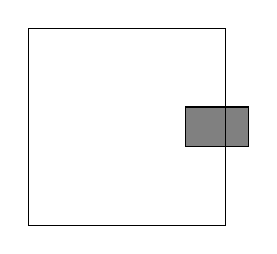
\begin{tikzpicture}	
			\filldraw [draw=black,fill=gray] (2, 1) rectangle (2.8, 1.5);
			\draw [draw=black] (0, 0) rectangle (2.5, 2.5);
		\end{tikzpicture}
		\caption{Informative update ($p$ strictly overlaps with the CS).}\label{fig1:informative-update}
	\end{subfigure}\hfill
	\begin{subfigure}[b]{.23\linewidth}
		\centering
		
\begin{tikzpicture}	
			\filldraw [draw=black,fill=gray] (0, 0) rectangle (2.5, 2.5);
		\end{tikzpicture}
		\caption{Uninformative update ($p$ equal to the CS).}\label{fig1:uninformative-equal-update}
	\end{subfigure}\hfill
	\begin{subfigure}[b]{.23\linewidth}
		\centering
		
\begin{tikzpicture}	
			\filldraw [draw=black,fill=gray] (0, 0) rectangle (3, 3);
			\filldraw [draw=black,fill=gray] (0, 0) rectangle (2.5, 2.5);
		\end{tikzpicture}
		\caption{Uninformative update ($p$ containing the CS).}\label{fig1:uninformative-update}
	\end{subfigure}
	\caption{A few examples of informative and uninformative updates of the CS. The big squares represent the CS. The grey shapes refer to $p$, the proposition added to the CG (and intersected with the CS to update it).}\label{fig1:informative-assertions}
\end{figure}

\subsection{Dynamic Semantics}

So far, we have mainly considered ``simplex'' assertions that did not make use of operators, connectives or quantifiers. But what about sentences like those in (\ref{ex1:complex-assertions})? How should they interact with the Context Set?
\begin{exe}
	\ex \label{ex1:complex-assertions}
	\begin{xlist}
		\ex {Jo did not grow up in France.}
		\ex {Jo grew up in France or Belgium.}
		\ex {Jo grew up in France and Ed in Belgium.}
	\end{xlist}
\end{exe}

The simplest way to deal with these sentences, would be to compute their intension (the proposition they denote) based on the semantics of negation, disjunction, and conjunction, and then, intersect the resulting proposition with the Context Set. We will call this approach the naive ``bulk'' CS update. There is evidence, coming from the behavior of presuppositions, that this might not be the way to go, and that complex assertions should be added to the Context Set ``bit by bit'' \parencite{Heim1982,Heim1983a,Heim1983b}.

To see this, let us consider the pair in (\ref{ex1:presupposition-conj}). The sentences in (\ref{ex1:presupposition-conj}) are conjunctive and only vary in the order of their conjuncts. Additionally, one of their conjuncts contains the presupposition trigger \textit{too}, associated with the predicate \textit{grew up in France}. In the felicitous variant (\ref{ex1:presupposition-conj-good}), \textit{too} occurs in the second conjunct; in the the infelicitous variant (\ref{ex1:presupposition-conj-good}), \textit{too} occurs in the first conjunct. Intuitively, \textit{X too VP} imposes that whatever predicate \textit{VP} denotes be true of at least one individual different from the one \textit{X} denotes. This presupposition can be seen as a precondition on the Context Set (as defined prior to the update step). In the case of (\ref{ex1:presupposition-conj-good}) and (\ref{ex1:presupposition-conj-good}), \textit{Ed too grew up in France} then imposes that the Context Set at the time of the update entail that somebody other than Ed (e.g., Jo) grew up in France. 

\begin{exe}
	\ex \label{ex1:presupposition-conj}
	\begin{xlist}
		\ex[] {Jo grew up in France, and Ed too grew up in France.}\label{ex1:presupposition-conj-good}
		\ex[\#] {Ed too grew up in France, and Jo grew up in France.}\label{ex1:presupposition-conj-bad}
	\end{xlist}
\end{exe}

Let us attempt a naive ``bulk'' CS update with sentences (\ref{ex1:presupposition-conj-good})/(\ref{ex1:presupposition-conj-bad}). The first step is to compute (\ref{ex1:presupposition-conj-good})/(\ref{ex1:presupposition-conj-bad})'s presuppositions and (propositional) assertions. The CS, as defined prior to the utterance of (\ref{ex1:presupposition-conj-good})/(\ref{ex1:presupposition-conj-bad}), then gets updated, provided that it verifies (\ref{ex1:presupposition-conj-good})/(\ref{ex1:presupposition-conj-bad})'s presupposition. Let us start with (\ref{ex1:presupposition-conj-good}) and (\ref{ex1:presupposition-conj-bad})'s presuppositional component. We can assume that the presupposition that somebody other than Ed grew up in France projects from inside the conjunctive operator. Under this assumption, both (\ref{ex1:presupposition-conj-good}) and (\ref{ex1:presupposition-conj-bad}) end up imposing that the CS prior to their utterance entail that somebody other than Ed grew up in France. This will in principle \textit{not} be verified. So, the naive ``bulk'' Context Set update correctly predicts the infelicity of (\ref{ex1:presupposition-conj-bad}), but, also, incorrectly predicts (\ref{ex1:presupposition-conj-good}) to be odd. Assuming the presupposition does not project does not address the issue. Under this assumption, both (\ref{ex1:presupposition-conj-good}) and (\ref{ex1:presupposition-conj-bad}) end up being presuppositionless, and the naive ``bulk'' CS update correctly predicts (\ref{ex1:presupposition-conj-good})'s felicity, but also incorrectly predicts (\ref{ex1:presupposition-conj-bad}) to be just as felicitous. So, regardless of how presupposition should exactly behave in complex sentences, the asymmetry between (\ref{ex1:presupposition-conj-good}) and (\ref{ex1:presupposition-conj-bad}) does not seem to be captured by the naive ``bulk'' CS update. 

The linear asymmetry in (\ref{ex1:presupposition-conj}) in fact suggests an alternative, ``bit by bit'' update strategy for complex sentences like conjunctions. If each conjunct were to update the CS one at a time, following the linear order of the sentence, then, the first conjunct of (\ref{ex1:presupposition-conj-good}) would create an updated CS that would incorporate the information that \textit{Jo grew up in France}, and as such verify the presupposition of (\ref{ex1:presupposition-conj-good})'s second conjunct (that somebody other than Ed grew up in France). This would allow (\ref{ex1:presupposition-conj-good})'s second conjunct to be subsequently intersected to the CS, and would predict the whole conjunction in (\ref{ex1:presupposition-conj-good}) to be felicitous. By contrast, (\ref{ex1:presupposition-conj-bad})'s first conjunct would still be problematic in this framework, because its presupposition would not be satisfied by the original CS. 

In this toy example, a presupposition was used as a diagnostic to better determine the nature of the CS update triggered by a conjunctive sentence. The conclusion is that the update should be dynamic: the two conjuncts should be intersected with the CS one by one, in the order in which they appear. This should apply to presuppositionless sentences as well; and is summarized in (\ref{ex1:conj-cs-update}). 


\begin{exe}
	\ex {\textsc{\textbf{Conjunctive update of the CS}}. Let $\mathcal{C}$ be a conversation and $CS(\mathcal{C})$ its Context Set. If a sentence $S$ of the form $X \wedge Y$, with $\llbracket X\rrbracket = p$ and $\llbracket Y\rrbracket = q$ is uttered, then a new Context Set $CS''(\mathcal{C})$ is derived by, first intersecting $CS(\mathcal{C})$ with $p$ to create $CS'(\mathcal{C})$, and second, intersecting $CS'(\mathcal{C})$ with $q$ to create $CS''(\mathcal{C})$:\\
		$CS''(\mathcal{C}) = (CS(\mathcal{C}) \cap p) \cap q = CS'(\mathcal{C})\cap q$\\
	The potential presuppositions of $X$ and $Y$ are tested on the CS at the time of their respective update, i.e. on $CS(\mathcal{C})$ and $CS'(\mathcal{C})$ respectively.}\label{ex1:conj-cs-update}
\end{exe}

\textit{Dynamic Semantics} is a framework that proposes to extend this view to other kinds of complex sentences, e.g. disjunctive and conditional sentences. In Dynamic Semantics, sentences give rise to different kinds of CS updates, depending on how they are constructed. More fundamentally, Dynamic Semantics proposes a shift of perspective when it comes to the meaning of assertions: assertions no longer denote propositions, instead they denote proposals to update the CS in specific ways. In that sense, assertions can be seen as functions from an input CS, to an output CS--sometimes called Context-Change Potentials (\textbf{CCP}). CCPs for disjunctive and conditional sentences are spelled out in (\ref{ex1:disj-cs-update}) and (\ref{ex1:cond-cs-update}) respectively.

\begin{exe}
	\ex {\textsc{\textbf{Disjunctive update of the CS}}. Let $\mathcal{C}$ be a conversation and $CS(\mathcal{C})$ its Context Set. If a sentence $S$ of the form $X \vee Y$, with $\llbracket X\rrbracket = p$ and $\llbracket Y\rrbracket = q$ is uttered, then a new Context Set $CS'(\mathcal{C})$ is derived by intersecting $CS(\mathcal{C})$ with $p \cup q$:\\
		$CS'(\mathcal{C}) = CS(\mathcal{C}) \cap (p \cup q)$\\
		The potential presuppositions of $X$ and $Y$ are tested on, respectively, $CS(\mathcal{C})$ and $CS(\mathcal{C}) \cap \neg p$.\footnote{There is a debate on whether or not disjunctions should behave symmetrically w.r.t. the presupposition(s) carried by their disjuncts. An alternative, symmetric way to evaluate $X$ and $Y$'s potential presuppositions, would be to test them against $CS(\mathcal{C}) \cap \neg q$ and $CS(\mathcal{C}) \cap \neg p$ respectively.}}\label{ex1:disj-cs-update}
	\ex {\textsc{\textbf{Conditional update of the CS}}. Let $\mathcal{C}$ be a conversation and $CS(\mathcal{C})$ its Context Set. If a sentence $S$ of the form \textit{if $X$ then $Y$}, with $\llbracket X\rrbracket = p$ and $\llbracket Y\rrbracket = q$ is uttered, then a new Context Set $CS''(\mathcal{C})$ is derived by, first intersecting $CS(\mathcal{C})$ with $p$ to create $CS'(\mathcal{C})$, and second, intersecting $CS'(\mathcal{C})$ with $q$ to create $CS''(\mathcal{C})$:\\
		$CS''(\mathcal{C}) = (CS(\mathcal{C}) \cap p) \cap q = CS'(\mathcal{C})\cap q$\\
		The potential presuppositions of $X$ and $Y$ are tested on the CS at the time of their respective update, i.e. on $CS(\mathcal{C})$ and $CS'(\mathcal{C})$ respectively.}\label{ex1:cond-cs-update}
\end{exe}


This incremental view of assertions leads to a revised, incremental definition of informativity, given in (\ref{ex1:informativity-ccp}). 

\begin{exe}
	\ex {\textsc{\textbf{Informativity}} (CCP view). A sentence $S$ is informative in a conversation $\mathcal{C}$, iff all the updates of $CS(\mathcal{C})$ it gives rise to are non-vacuous.}\label{ex1:informativity-ccp}
\end{exe}

In sum, assertions can be seen as proposals to update (shrink) the CS. The specific update they give rise to is compositionally derived, and incrementally performed, following the structure of the sentence. We will use a similar approach in Chapter \ref{chap:accommodating-quds} when defining questions \textit{evoked} by assertions. But this first requires to define what questions mean. This is what we do in the next section, in which we show that questions influence, not the size, but rather, the topology of the CS.








\section{Questions indicate which kind of information is worth providing}\label{sec:questions}

\subsection{Questions as answerhood conditions}
Participants in a conversation utter assertions to shrink the CS, and hopefully, jointly figure out which world they are in. But this allows for very unnatural interactions like (\ref{ex1:weird-assertion-sequence}), taking the forms of sequences of intuitively unrelated sentences--as long as each of them denotes propositions shrinking the CS!

\begin{exe}
	\ex {--Jo grew up in France.\\
		--I like cheese.\\
		--Al is arriving tomorrow.}\label{ex1:weird-assertion-sequence}
\end{exe}

This is where questions enter the game. Intuitively, a question indicates an interest in \textit{which} proposition(s) hold, among a restricted set. The proposition at stake are typically possible answers to the question \cite{Hamblin1973,Dayal1996}. Questions therefore denote sets of sets of worlds (equivalent to a type $\langle\langle \texttt{s}, \texttt{t}\rangle, \texttt{t}\rangle$), and constrain which kind of (informative) propositions can be uttered as a follow-up. For instance, a polar question such as \textit{Is it raining?} will typically request information of the form \textit{It is raining}, or \textit{It is not raining}, see (\ref{ex1:simple-polar-q}). 

\begin{exe}
	\ex {--Is it raining?\\
	--Yes, it is raining. / No, it is not raining.}\label{ex1:simple-polar-q}
\end{exe} 

The question \textit{Is it raining?} can thus be represented as a set made of two propositions, namely, the proposition that \textit{it is raining}, and the proposition that \textit{it is not raining}.  

\begin{exe}
	\ex {$\llbracket$ Is it raining? $\rrbracket$ = $\lbrace$ $\llbracket$ It is raining $\rrbracket$, $\llbracket$ It is not raining $\rrbracket$ $\rbrace$\\
		\phantom{$\llbracket$ Is it raining? $\rrbracket$} = $\lbrace\lambda w. \ $ it is raining in $w$, $ \ \lambda w. \ $ it is not raining in $w \rbrace$\\
	\phantom{$\llbracket$ Is it raining? $\rrbracket$} : $\langle\langle \texttt{s}, \texttt{t}\rangle, \texttt{t}\rangle$}
\end{exe}

In the case of the question \textit{is it raining?}, the set of possible answers is fairly simple: it only contains two elements. These two elements  cover the space of all possibilities,\footnote{This is the case assuming there is no vagueness-induced ``grey area'', i.e. any salient situation is either a \textit{raining}-situation, or a \textit{not raining}-situation} and are \textit{exclusive}: if it's the case that it's raining (at a salient place, at a salient time) in $w$, then, it's not the case that it is not raining (at the same place, at the same time), in $w$. We will see in the next section that this configuration amounts to a partition of the CS. A definition of exclusivity under the set interpretation of propositions is given in (\ref{ex1:proposition-exclusivity}).

\begin{exe}
	\ex {\textsc{\textbf{Exclusive propositions}}. $p : \langle \texttt{s}, \texttt{t}\rangle$ and $q : \langle \texttt{s}, \texttt{t} \rangle$ are exclusive if $p \cap q = \emptyset$.}\label{ex1:proposition-exclusivity}
\end{exe}


But questions may not always intuitively request information about exclusive propositions. For instance, a \textit{wh}-question like \textit{Which students passed the class?} expects answers that convey a subset of students who passed the class, see (\ref{ex1:simple-wh-q}). But there are many possible, overlapping subsets of students, so, the corresponding propositions will be overlapping as well. For instance, the proposition that \textit{Jo passed the class}, denotes the set of worlds in which Jo passed the class, and this set happens to contain the set of worlds where both Jo and Al passed the class. It also overlaps with the set of worlds in which Al passed the class. 

\begin{exe}
	\ex {Which students passed the class?\\
	--Jo did.\\
	--Al did.\\
	--Jo and Al did.}\label{ex1:simple-wh-q}
\end{exe} 

We will call propositions like \textit{Jo passed the class}, and \textit{Jo and Al passed the class}, alternatives associated to the question \textit{Which students passed the class?} Alternatives may be overlapping; and, as we will see, can be obtained from the original question by substituting its \textit{wh}-component (e.g., \textit{which students}), with relevant, same-type material (e.g., students or groups of students).\footnote{It is worth mentioning that the set $\lbrace\lambda w. $ it is raining in $w$, $ \ \lambda w. $ it is not raining in $w \rbrace$ does not strictly speaking correspond to the set of alternatives raised by \textit{Is it raining?} Section \ref{sec:q-derivation} further specifies how alternatives get compositionally derived, and predicts that \textit{Is it raining?} should only give rise to one alternative: $\lambda w. $ it is raining in $w$. The set $\lbrace\lambda w. $ it is raining in $w$, $ \ \lambda w. $ it is not raining in $w \rbrace$ is derived from this singleton alternative \textit{via} the ``pragmatic'' process presented in (\ref{ex1:partition-induced}), in the next Section.}


\begin{exe}
	\ex {Question : $\llbracket$ Which students passed the class? $\rrbracket$\\
		Alternatives: $\lbrace\llbracket$ Jo passed $\rrbracket$, $\llbracket$ Al passed $\rrbracket$, $\llbracket$ Jo and Al passed $\rrbracket$ ... $\rbrace$}
\end{exe}


Why would this overlap between alternative answers be an issue in modeling the meaning of questions? The fact that entailing or merely overlapping propositions should be considered equally good answers does not capture the idea that more specific propositions constitute more exhaustive answers than less specific ones. For instance, answering that \textit{Jo passed}, in theory leaves the fate of the other students undecided--for instance, it does not settle if \textit{Al passed}, or not. Answering that \textit{Jo and Al passed} by contrast, settles Al's fate, in addition to Jo's. Ideally, an answer to \textit{Which students passed?} should explicitly address whether \textit{each} student of the class passed, or not. That would be an exhaustive answer.

\subsection{Questions as partitions of the Context Set}

We have just discussed that, at the semantic level, questions characterize the conditions under which they are answered, i.e. denote a set of potentially overlapping propositions. But, just like we did with assertions, the effect of this semantics on the Context Set has to be defined. There is in fact a deterministic way to change a set of overlapping propositions $P$ (i.e. a set of subsets of the CS), into a set of exclusive subsets of the CS (called \textit{cells}, for reasons made clear in (\ref{ex1:partition-induced})). To do so, one can group in the same cell the worlds of the Context Set that all ``agree'' on all propositions in $P$. This ``agreement'' property amounts to the same-cell relation in (\ref{ex1:same-cell}). This relation is reflexive, symmetric and transitive, i.e. is an equivalence relation (see proof in (\ref{ex1:cell-equiv-relation})). From this, we can conclude that the set of subsets of the CS induced by $P$, obtained by grouping worlds of the CS according to the same-cell relation, forms a partition of the Context Set (see proof in (\ref{ex1:partition-induced})).\footnote{Cells as we defined them are also called equivalence classes. It's a general property that equivalence classes induced by an equivalence relation on a certain set on which this relation is defined, will create a partition of the set.} So, on top of being exclusive, cells are non-empty and together cover the CS. We assume that the process changing the set of alternative propositions raised by a question, to a partition of the CS, belongs to pragmatics. So, questions \textit{denote} sets of alternative propositions, and this set \textit{pragmatically induces} a partition structure on the CS.

\begin{exe}
	\ex {\textsc{\textbf{Same-cell relation}} ($\equiv_P$.). Let $P$ be a set of propositions, i.e. a set of subsets of the Context Set ($P \in \mathcal{P}(\mathcal{P}(CS))$, with $\mathcal{P}$ the powerset operation). Let $w$ and $w'$ be two worlds of the Context Set. $w \equiv_{P} w'$ iff, $\forall p \in P. \  p(w) = p(w')$.}\label{ex1:same-cell}
		\ex {$\equiv_P$ is an equivalence relation, no matter what $P$ is. Let $\forall P \in \mathcal{P}(\mathcal{P}(CS))$.
		\begin{itemize}
			\item $\equiv_P$ is reflexive: $\forall w \in CS. \ \forall p \in P. \  p(w) = p(w)$.
			\item $\equiv_P$ is symmetric. Let $\forall (w, w') \in CS^2$.\\ $\forall p \in P. \  p(w) = p(w')$ iff $\forall p \in P. \  p(w') = p(w)$.
			\item $\equiv_P$ is transitive. Let $\forall (w, w', w'') \in CS^3$.\\
			We assume $\forall p \in P. \  p(w) = p(w')$ and $\forall p \in P. \  p(w') = p(w'')$.\\Let $\forall p \in P$. 
			We have $p(w) = p(w')$ and $p(w') = p(w'')$, so $p(w') = p(w'')$.\\
			So, $\forall p \in P. \  p(w) = p(w'')$
	\end{itemize}}\label{ex1:cell-equiv-relation}
	\ex {\textsc{\textbf{Partition of the CS induced by $P$}}.\footnote{\textcite{Fox2018} proposes an alternative way to derive a partition of the CS from a set of alternative propositions, leveraging the covert operator \textit{exh}} Let $P$ be a set of propositions. The partition induced by $P$ in the Context Set is the set of subsets of the CS (cells): $\mathfrak{P}_{P, CS} =  \lbrace \lbrace w' \ | \ w' \in CS \wedge w' \equiv_P w \rbrace \ | \ w \in CS\rbrace$. This set partitions the CS.
	\begin{itemize}
		\item No cell $c$ of $\mathfrak{P}_{P, CS}$ is empty. Let $c \in \mathfrak{P}_{P, CS}$. There is a $w \in CS$ s.t. $c = \lbrace w' \ | \ w' \in CS \wedge w' \equiv_P w \rbrace$. Then at least $w \in c$, because $w \equiv_P w$.
		\item Cells cover the CS. Let $w \in CS$. $\mathfrak{P}_{P, CS}$ contains a cell $c = \lbrace w' \ | \ w' \in CS \wedge w' \equiv_P w \rbrace$. Then $w \in c$ because $w \equiv_P w$.
		\item Cells are disjoint. Let $(c, c') \in \mathfrak{P}_{P, CS}$, s.t. $c \cap c' \neq \emptyset$. We show $c = c'$. $c$ and $c'$ have resp. the form $c = \lbrace w'' \ | \ w'' \in CS \wedge w'' \equiv_P w \rbrace$ and $c = \lbrace w'' \ | \ w'' \in CS \wedge w'' \equiv_P w' \rbrace$, for $(w, w') \in CS^2$. Let $w''' \in c \cap c'$. Then $w''' \equiv_P w$ and $w''' \equiv_P w'$, and so by symmetry and transitivity, $w \equiv_P w'$, and $c=c'$.
		\end{itemize}}\label{ex1:partition-induced}
\end{exe}

It is easy to show that, in the polar example (\ref{ex1:simple-polar-q}), the subsets of the CS defined by \textit{It is raining} and \textit{It is not raining}, which we said were intuitive answers to the question, form a partition of the CS. Section \ref{sec:q-derivation} will in fact show that polar questions of the form $p?$ \textit{denote} the singleton set formed by $p$, and \textit{induce} a $2$-cell partition of the form $\lbrace p, \neg p\rbrace$.


Let us now see how the above definitions apply to a \textit{wh}-question like \textit{Which students passed?} in (\ref{ex1:simple-wh-q}). Let's assume there are only two salient students, Jo and Al. We assume that the alternatives the question raises (labeled $P$), are the proposition that \textit{Jo passed}, and the proposition that \textit{Al passed}. We assume that the CS contains six possible worlds, which vary according to whether Jo, Al, both, or none passed the class. The worlds may vary in other respects, that are not relevant to us here. The alternatives and cells associated with this question are given in (\ref{ex1:wh-partition-computation}). The alternative set $P$ then corresponds to two subsets of the CS, which do not cover it. In particular, the world in which nobody passed ($w_0$) is included in none of the two alternatives. Moreover, the two subsets are overlapping: both \textit{Jo passed} and \textit{Al passed} contain $w_4$, $w_5$, and $w_6$. Now turning to the cells induced by $P$ on the CS, we notice that there are four of them, which correspond to worlds where nobody, only Jo, only Al, or both Jo and Al passed the class. Such cells cover the CS, are disjoint, and non-empty, so correctly form a partition of the CS. They also fully specify, for \textit{both} Jo and Al, if they passed the class; and as such constitute exhaustive answers to the original question.

\begin{exe}
	\ex {Question : \textit{Which students passed the class?}\\
	Context Set: $\lbrace w_0, w_1, w_2, w_3, w_4, w_5, w_6\rbrace$, s.t.:
	\begin{itemize}
		\item Nobody passed in $w_0$;
		\item Only Jo passed in $w_1$ and $w_2$;
		\item Only Al passed in $w_3$;
		\item Both Jo and Al passed in $w_4$, $w_5$, and $w_6$.
	\end{itemize}
	Alternatives ($P$): $\lbrace$$\llbracket$Jo passed$\rrbracket$, $\llbracket$Al passed$\rrbracket$$\rbrace$ = $\lbrace \lbrace w_1, w_2, w_4, w_5, w_6\rbrace, \lbrace w_3, w_4, w_5, w_6 \rbrace\rbrace$\\
	Cells induced by $\equiv_P$: $\lbrace \lbrace w_0\rbrace, \lbrace w_1, w_2 \rbrace, \lbrace w_3 \rbrace, \lbrace w_4, w_5, w_6\rbrace\rbrace$
	}\label{ex1:wh-partition-computation}
\end{exe}
\begin{figure}[H]
	\centering
		\begin{subfigure}[t]{.27\linewidth}
		\centering
		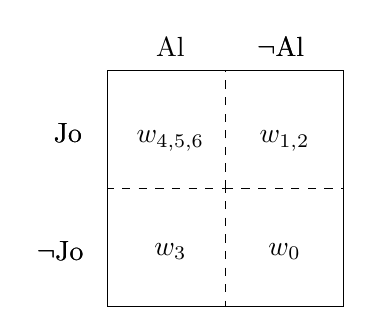
\begin{tikzpicture}	
			\node[] at(.8, 3.3) {Al};
			\node[] at(2.2, 3.3) {$\neg$Al};
			\node[] at(-.6, .7) {$\neg$Jo};
			\node[] at(-.5, 2.2) {Jo};
			
			\node[] at(.8,2.1) {$w_{4, 5, 6}$};
			\node[] at(2.25,2.1) {$w_{1, 2}$};
			\node[] at(.8,.7) {$w_{3}$};
			\node[] at(2.25,.7) {$w_{0}$};
			
			\node[] at(2.2, 3.3) {$\neg$Al};
			\node[] at(-.6, .7) {$\neg$Jo};
			\node[] at(-.5, 2.2) {Jo};
			\draw [draw=black] (0, 0) rectangle (3, 3);
			\draw [draw=black,dashed] (0, 0) rectangle (1.5, 1.5);
			\draw [draw=black, dashed] (1.5, 1.5) rectangle (3, 3);
		\end{tikzpicture}
		\caption{Distribution of $w_0 ... w_6$ in the CS.}\label{fig1:cs-worlds}
	\end{subfigure}\hfill
	\begin{subfigure}[t]{.27\linewidth}
		\centering
		\begin{tikzpicture}	
			\node[] at(.8, 3.3) {Al};
			\node[] at(2.2, 3.3) {$\neg$Al};
			\node[] at(-.6, .7) {$\neg$Jo};
			\node[] at(-.5, 2.2) {Jo};
			\draw [draw=black] (0, 0) rectangle (3, 3);
			\draw [draw=black,pattern=north west lines] (0, 0) rectangle (1.5, 3);
			\draw [draw=black,pattern=north east lines] (0,1.5) rectangle (3, 3);
		\end{tikzpicture}
		\caption{Alternatives: \begin{tikzpicture}
				\draw [draw=black,pattern=north west lines] (0, 0) rectangle (.5, .3);
		\end{tikzpicture} defines \textit{Al passed} and \begin{tikzpicture}
		\draw [draw=black,pattern=north east lines] (0, 0) rectangle (.5, .3);
		\end{tikzpicture} defines \textit{Jo passed}.}\label{fig1:alternatives}
	\end{subfigure}\hfill
	\begin{subfigure}[t]{.41\linewidth}
		\centering
		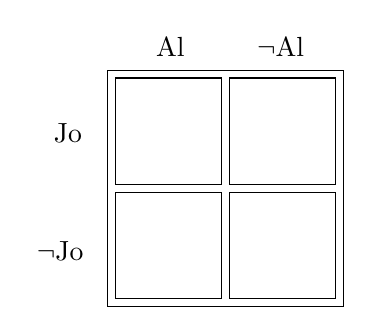
\begin{tikzpicture}	
			\node[] at(.8, 3.3) {Al};
			\node[] at(2.2, 3.3) {$\neg$Al};
			\node[] at(-.6, .7) {$\neg$Jo};
			\node[] at(-.5, 2.2) {Jo};
			\draw [draw=black] (0, 0) rectangle (3, 3);
			\draw [draw=black] (0.1, 1.55) rectangle (1.45, 2.9);
			\draw [draw=black] (1.55, 0.1) rectangle (2.9, 1.45);
			\draw [draw=black] (0.1, 0.1) rectangle (1.45, 1.45);
			\draw [draw=black] (1.55, 1.55) rectangle (2.9, 2.9);
		\end{tikzpicture}
		\caption{Partition induced by \begin{tikzpicture}
				\draw [draw=black,pattern=north west lines] (0, 0) rectangle (.5, .3);
			\end{tikzpicture} and \begin{tikzpicture}
				\draw [draw=black,pattern=north east lines] (0, 0) rectangle (.5, .3);
		\end{tikzpicture}. Cells correspond to the subsets of Figure \ref{fig1:alternatives} featuring the same overall pattern. }\label{fig1:cells}
	\end{subfigure}
\caption{Partitioning of the CS defined in (\ref{ex1:wh-partition-computation}) according to the alternatives \textit{Jo passed} and \textit{Al passed}. The CS is organized as follows: counter-clockwise, quadrant I is made of \textit{Jo but not Al}-worlds; quadrant II, \textit{Jo and Al}, quadrant III, \textit{Al but not Jo}, and quadrant IV, \textit{neither Jo nor Al}.}
\end{figure}


To summarize, at the pragmatic level questions are partitions of the Context Set, as formalized in (\ref{ex1:question-partition}).\footnote{It is important to note that questions may be taken to have a partition \textit{semantics}. But we do not cover this here.} The cells of such partitions constitute maximal answers to the questions. Unions of two or more cells constitute non-maximal answers, as defined in (\ref{ex1:question-answer}).

\begin{exe}
	\ex {\textsc{\textbf{Standard semantics for questions}} \parencite{Jager1996,Hulstijn1997,Groenendijk1984,Groenendijk1999}.	Given a conversation $\mathcal{C}$ and a Context Set $CS(\mathcal{C})$, a question on $CS(\mathcal{C})$ is a partition of $CS(\mathcal{C})$, i.e. a set of subsets of $CS(\mathcal{C})$ (``cells'') $\lbrace c_1, ..., c_k\rbrace$ s.t.:
		\begin{itemize}
			\item ``No empty cell'': $\forall i \in [1; k]. \ c_i \neq \emptyset$
			\item ``Full cover'': $\bigcup_{i\in[1;k]} c_i = CS(\mathcal{C})$
			\item ``Pairwise disjointness'': $\forall (i, j) \in [1;k]^2. \ i \neq j \Rightarrow c_i \cap c_j = \emptyset$
		\end{itemize}
	}\label{ex1:question-partition}
	\ex {\textsc{\textbf{Answers to a question}}. Given a conversation $\mathcal{C}$, a Context Set $CS(\mathcal{C})$, and a question $Q$ forming a partition $\lbrace c_1, ..., c_k\rbrace$ of $CS(\mathcal{C})$:
		\begin{itemize}
			\item Any $c \in \lbrace c_1, ..., c_k\rbrace$ constitutes a maximal answer to $Q$;
			\item Any $c'$ s.t. $\exists C \subseteq \lbrace c_1, ..., c_k\rbrace. \ |C| > 1 \wedge c' = \bigcup C$ is a non-maximal answer to $Q$.
		\end{itemize}
	}\label{ex1:question-answer}
\end{exe}

Just like we did with assertions, let us clarify further what it means to be a good question. We have established that the idea of a partition is a good candidate to model the effect of questions on a given CS. But what if the CS is already such that the partition induced by the question's alternatives is just made of one big cell? Such a configuration suggests that the question is already \textit{settled}, meaning, the CS already makes one maximal answer trivial. For instance, if it is already common ground between the conversation's participants that \textit{it is raining} (at the salient place and time) in (\ref{ex1:simple-polar-q}), then, the question \textit{Is it raining?} appears completely trivial. This is illustrated in Figure \ref{fig1:trivial-q} and generalized in (\ref{ex1:trivial-question}).


\begin{figure}[H]
	\centering
	\begin{subfigure}[t]{.27\linewidth}
		\centering
		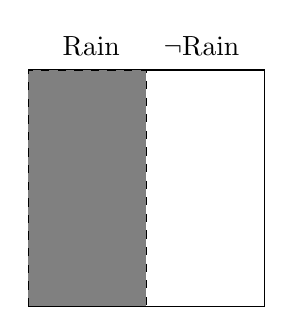
\begin{tikzpicture}	
			\node[] at(.8, 3.3) {Rain};
			\node[] at(2.2, 3.3) {$\neg$Rain};
			\draw [draw=black] (0, 0) rectangle (3, 3);
			\filldraw [draw=black,dashed,fill=gray] (0, 0) rectangle (1.5, 3);
		\end{tikzpicture}
		\caption{Interecting the proposition that \textit{It's raining} (
\begin{tikzpicture}
				\filldraw [draw=black,fill=gray] (0, 0) rectangle (.5, .3);
			\end{tikzpicture}) with a CS that is agnostic about the weather.}\label{fig1:cs-raining-not-raining}
	\end{subfigure}\hfill
	\begin{subfigure}[t]{.27\linewidth}
		\centering
		\begin{tikzpicture}	
			\node[] at(.8, 3.3) {Rain};
			\draw [draw=black,pattern=north west lines] (0, 0) rectangle (1.5, 3);
		\end{tikzpicture}
		\caption{Alternatives on the restricted CS: \begin{tikzpicture}
				\draw [draw=black,pattern=north west lines] (0, 0) rectangle (.5, .3);
			\end{tikzpicture} defines \textit{It's raining}.}\label{fig1:alternatives-raining}
	\end{subfigure}\hfill
	\begin{subfigure}[t]{.36\linewidth}
		\centering
		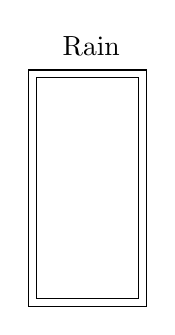
\begin{tikzpicture}	
			\node[] at(.8, 3.3) {Rain};
			\draw [draw=black] (0, 0) rectangle (1.5, 3);
			\draw [draw=black] (0.1, 0.1) rectangle (1.4, 2.9);
		\end{tikzpicture}
		\caption{Partition induced by \begin{tikzpicture}
				\draw [draw=black,pattern=north west lines] (0, 0) rectangle (.5, .3);
			\end{tikzpicture} on the CS. Cells correspond to the subsets of Figure \ref{fig1:alternatives-raining} featuring the same overall pattern ($1$ such subset).}\label{fig1:cells-raining}
	\end{subfigure}
	\caption{Updating the CS with the proposition that \textit{It's raining}, and then computing the partition induced by \textit{Is it raining} on the resulting ``shrunk'' CS. The outcome is a single-cell partition, i.e., the question has a trivial pragmatics.}\label{fig1:trivial-q}
\end{figure}


\begin{exe}
	\ex {\textsc{\textbf{Trivial Question}}. Let $\mathcal{C}$ be a conversation, $CS(\mathcal{C})$ its associated Context Set, and $Q$ a question. $Q$ is trivial given $CS(\mathcal{C})$ iff the partition induced by $Q$ on $CS(\mathcal{C})$ is made of a singleton cell, i.e. has cardinal $1$.}\label{ex1:trivial-question}
\end{exe}

We now have a basic notion of what it mean to be a good assertion, given a CS, and a good question, given a CS. A good assertion has to be informative, i.e. properly shrink the CS (as per (\ref{ex1:informativity})/(\ref{ex1:informativity-ccp})). A good question has to induce a non-trivial, multiple-cell partition on the CS (as per (\ref{ex1:trivial-question})). But being a good question or a good assertion, does not \textit{only} depend on the state of the CS! In particular, good assertions also have to be good answers to good questions. This principle, dubbed \textit{Question-Answer Congruence}, is given in (\ref{ex1:q-a-congruence}).

\begin{exe}
	\ex {\textsc{\textbf{Question-Answer Congruence}} \parencite{Katzir2015}. A felicitous assertion has to be a good answer to a good question.}\label{ex1:q-a-congruence}
\end{exe}

The next Section presents what can be seen as a partial implementation of this principle, in the form of a general principle dubbed \textsc{Relevance}. It also points out the limitations of this principle.


\section{Assertions as good answers to questions}\label{sec:q-a-interaction}

\subsection{Relevance mediates questions and assertions}
Now that we precisified what assertions and questions are, it becomes possible to (at least partially) define what a good assertion should be, given a question. The principles we introduce in this Section are based on the general concept of \textsc{Relevance}. They will eventually rule out informative but ``unnatural'' sequences of assertions like (\ref{ex1:weird-assertion-sequence}), but also, more generally, a wide range of odd question-answer pairs.

Following much previous literature \parencite{VanKuppevelt1995a,VanKuppevelt1995b,Roberts1996,Roberts2012,Ginzburg1996,Buring2003}, we call the question against which assertions are evaluated, \textit{Question under Discussion} (henceforth \textbf{QuD}). QuDs are typically seen as partitions of the CS. In
(\ref{ex1:question-answer}), we defined cells an unions of cells as respectively maximal and non-maximal answers to a question. Very broadly, \textsc{Relevance} constrains what a proposition should do to the cells of the QuD. Let us now unpack this with an example.

If for instance the QuD is about which country Jo grew up in (as in (\ref{ex1:qud-country})), the CS will be partitioned according to propositions of the form \textit{Jo grew up in c}, with \textit{c} a country. Utterances such as (\ref{ex1:france-relevant}) or (\ref{ex1:france-belgium-relevant}), both seem relevant to that kind of QuD, and both constitute answers to the QuD--maximal, or not. By contrast, utterances such as (\ref{ex1:native-irrelevant}), (\ref{ex1:wine-irrelevant}) or (\ref{ex1:cat-irrelevant}), do not appear relevant, and do \textit{not} constitute answers to the QuD: there are native and non-native French speakers in virtually all countries; same holds for wine-lovers and wine-haters; as for (\ref{ex1:cat-irrelevant}) it seems completely independent from the subject matter.\footnote{It is interesting to note that (\ref{ex1:native-irrelevant}) and (\ref{ex1:wine-irrelevant}) can be more easily coerced into relevance than (\ref{ex1:cat-irrelevant}). For instance with (\ref{ex1:native-irrelevant}), one might consider that France is the country which, in proportion, comprises the most native French speakers, and so (\ref{ex1:native-irrelevant}) may be understood as \textit{It is likely that Jo grew up in France}--which constitutes a modalized answer to the QuD. This kind of reasoning is harder (if not impossible) to perform when facing an utterance like (\ref{ex1:cat-irrelevant}).} These various configurations are sketched in Figure \ref{fig1:relevance-example}.

\begin{exe}
	\ex {QuD: In which country did Jo grow up?}\label{ex1:qud-country}
	\begin{xlist}
		\ex[] {Jo grew up in France.}\label{ex1:france-relevant}
		\ex[] {Jo grew up in France or Belgium.}\label{ex1:france-belgium-relevant}
		\ex[??] {Jo speaks French natively.}\label{ex1:native-irrelevant}
		\ex[??] {Jo enjoys wine.}\label{ex1:wine-irrelevant}
		\ex[\#] {The cat went outside.}\label{ex1:cat-irrelevant}
	\end{xlist}
\end{exe}

\begin{figure}[H]
	\centering
	\begin{subfigure}[t]{.24\linewidth}
		\centering
		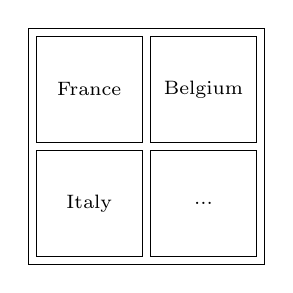
\begin{tikzpicture}	
			\draw [draw=black] (0, 0) rectangle (3, 3) ;
			\draw [draw=black] (0.1, 1.55) rectangle (1.45, 2.9) node[pos=.5] {\scriptsize France};
			\draw [draw=black] (1.55, 0.1) rectangle (2.9, 1.45) node[pos=.5] {\scriptsize ...};
			\draw [draw=black] (0.1, 0.1) rectangle (1.45, 1.45) node[pos=.5] {\scriptsize Italy};
			\draw [draw=black] (1.55, 1.55) rectangle (2.9, 2.9) node[pos=.5] {\scriptsize Belgium};
		\end{tikzpicture}
		\caption{QuD for \textit{In which city did Jo grow up?}}
	\end{subfigure}\hfill
		\begin{subfigure}[t]{.24\linewidth}
			\centering
		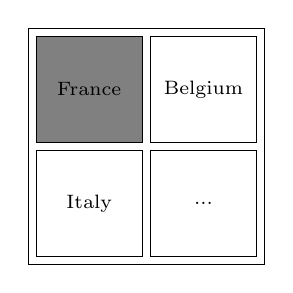
\begin{tikzpicture}	
			\draw [draw=black] (0, 0) rectangle (3, 3) ;
			\filldraw [draw=black,fill=gray] (0.1, 1.55) rectangle (1.45, 2.9) node[pos=.5] {\scriptsize France};
			\draw [draw=black] (1.55, 0.1) rectangle (2.9, 1.45) node[pos=.5] {\scriptsize ...};
			\draw [draw=black] (0.1, 0.1) rectangle (1.45, 1.45) node[pos=.5] {\scriptsize Italy};
			\draw [draw=black] (1.55, 1.55) rectangle (2.9, 2.9) node[pos=.5] {\scriptsize Belgium};
		\end{tikzpicture}
		\caption{Utterance: \textit{Jo grew up in France}.}
	\end{subfigure}\hfill
	\begin{subfigure}[t]{.24\linewidth}
		\centering
		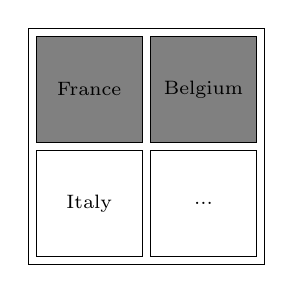
\begin{tikzpicture}	
			\draw [draw=black] (0, 0) rectangle (3, 3) ;
			\filldraw [draw=black,fill=gray] (0.1, 1.55) rectangle (1.45, 2.9) node[pos=.5] {\scriptsize France};
			\draw [draw=black] (1.55, 0.1) rectangle (2.9, 1.45) node[pos=.5] {\scriptsize ...};
			\draw [draw=black] (0.1, 0.1) rectangle (1.45, 1.45) node[pos=.5] {\scriptsize Italy};
			\filldraw [draw=black,fill=gray] (1.55, 1.55) rectangle (2.9, 2.9) node[pos=.5] {\scriptsize Belgium};
		\end{tikzpicture}
		\caption{Utterance: \textit{Jo grew up in France or Belgium}.}
	\end{subfigure}\hfill
	\begin{subfigure}[t]{.24\linewidth}
		\centering
		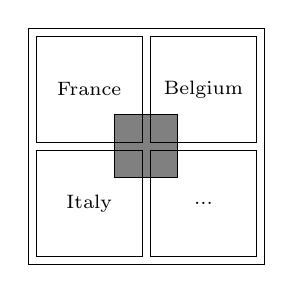
\begin{tikzpicture}	
			\draw [draw=black] (0, 0) rectangle (3, 3) ;
			\filldraw [draw=black,fill=gray] (1.1, 1.1) rectangle (1.9, 1.9) node[pos=.5] {};
			\draw [draw=black] (0.1, 1.55) rectangle (1.45, 2.9) node[pos=.5] {\scriptsize France};
			\draw [draw=black] (1.55, 0.1) rectangle (2.9, 1.45) node[pos=.5] {\scriptsize ...};
			\draw [draw=black] (0.1, 0.1) rectangle (1.45, 1.45) node[pos=.5] {\scriptsize Italy};
			\draw [draw=black] (1.55, 1.55) rectangle (2.9, 2.9) node[pos=.5] {\scriptsize Belgium};
		\end{tikzpicture}
		\caption{Utterance: (\ref{ex1:native-irrelevant}), (\ref{ex1:wine-irrelevant}) or (\ref{ex1:cat-irrelevant}).}
	\end{subfigure}
	\caption{QuD-utterance configurations for a QuD like \textit{In which country did Jo grow up}, and possible follow-up utterance.}\label{fig1:relevance-example}
\end{figure}

From this, we can conclude that a proposition is ``relevant'' to a question, if it constitutes a maximal or a non-maximal answer to the question. This is similar in spirit to the notion of \textit{Aboutness} developed \cite{Lewis1988}, according to which a proposition $p$ is about a subject matter (in modern terms, a QuD), if and only if the truth value of that proposition supervenes on that subject matter (i.e. $p$ should not introduce truth-conditional distinctions between cellmates, i.e. $p$ does not ``cut across'' cells). This is rephrased in (\ref{ex1:lewis-relevance}). 

\begin{exe}
	\ex\label{ex1:lewis-relevance} {\textsc{\textbf{\citeauthor{Lewis1988}'s Relevance}} (rephrased in the QuD framework). Let $\mathcal{C}$ be a conversation, $Q$ a QuD defined as a partition of $CS(\mathcal{C})$. Let $p$ be a proposition. $p$ is \textsc{\citeauthor{Lewis1988}-Relevant} to $Q$, iff $\exists C \subseteq Q. \ p \cap CS(\mathcal{C}) = C$}
\end{exe}


A typical \textsc{\citeauthor{Lewis1988}-Relevant} configuration is exemplified in Figure \ref{fig1:2-cells-relevant}. Note however two edge cases. The first, is that of a proposition whose intersection with the CS is empty (a contextual contradiction). This kind of proposition verifies (\ref{ex1:lewis-relevance}), because the empty set is a subset of any set, including the set of propositions defined by the QuD--whatever it is. Figure \ref{fig1:no-cell-relevant} exemplifies this kind of configuration. The second edge case, is that of a proposition whose intersection with the CS is the entire CS (a contextual tautology, uninformative as per (\ref{ex1:informativity})). This kind of proposition also verifies (\ref{ex1:lewis-relevance}), because the entire CS corresponds to the unions of all cells of any given QuD defined on that CS. Figure \ref{fig1:all-cells-relevant} exemplifies this kind of configuration. 

But, coming back to the QuD \textit{In which country did Jo grow up?}, what about an utterance of the form \textit{Jo grew up in Paris?} Although overinformative (the QuD was only asking about countries, not cities!), this utterance appears relevant, because it allows to infer that Jo grew up in France, and not, say, Belgium. This kind of configuration is sketched in Figure \ref{fig1:relevance-example-2}.

\begin{figure}[H]
	\centering
	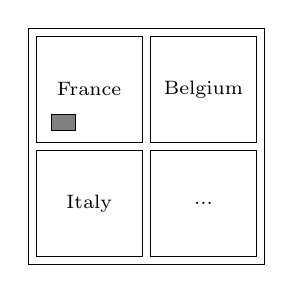
\begin{tikzpicture}	
		\draw [draw=black] (0, 0) rectangle (3, 3) ;
		\draw [draw=black] (0.1, 1.55) rectangle (1.45, 2.9) node[pos=.5] {\scriptsize France};
		\filldraw [draw=black,fill=gray] (0.3, 1.7) rectangle (0.6, 1.9) node[pos=.5] {};
		\draw [draw=black] (1.55, 0.1) rectangle (2.9, 1.45) node[pos=.5] {\scriptsize ...};
		\draw [draw=black] (0.1, 0.1) rectangle (1.45, 1.45) node[pos=.5] {\scriptsize Italy};
		\draw [draw=black] (1.55, 1.55) rectangle (2.9, 2.9) node[pos=.5] {\scriptsize Belgium};
	\end{tikzpicture}
	\caption{QuD-utterance configuration for a QuD like \textit{In which country did Jo grow up?} and an utterance like \textit{Jo grew up in Paris}.}\label{fig1:relevance-example-2}
\end{figure}

The view of relevance, developed by \textcite{Roberts2012}, captures this intuition, by stating that a relevant proposition has to rule out at least one maximal answer conveyed by the QuD. In other words, a relevant proposition has to be incompatible with at least one cell of the QuD. This is summarized in (\ref{ex1:roberts-relevance}). This definition makes uninformative propositions irrelevant (see Figure \ref{fig1:all-cells-relevant}), but allows certain propositions that do not coincide with the grand union of a subset of the QuD's cells, to be relevant (see Figures \ref{fig1:sub-cell-relevant} and \ref{fig1:sub-1-cell-relevant}). In other words, relevant propositions in the sense of \citeauthor{Roberts2012} may introduce truth-conditional distinctions between cellmates--as long as they rule out a cell. A particular case is that of propositions like \textit{Jo grew up in Paris}, when the QuD is about countries, which strictly entail a specific cell of the QuD, i.e. are strictly contained in one single cell (see Figure \ref{fig1:sub-cell-relevant}).


\begin{exe}
	\ex\label{ex1:roberts-relevance} {\textsc{\textbf{\citeauthor{Roberts2012}'s Relevance}} \parencite{Roberts2012}. Let $\mathcal{C}$ be a conversation, $Q$ a (non-trivial) QuD defined as a partition of $CS(\mathcal{C})$. Let $p$ be a proposition. $p$ is \textsc{\citeauthor{Roberts2012}-Relevant} to $Q$, if $\exists c \in Q. \ p \cap c = \emptyset$.
	}
\end{exe}


\begin{figure}[H]
	\centering
	\begin{subfigure}[b]{.3\linewidth}
		\centering
		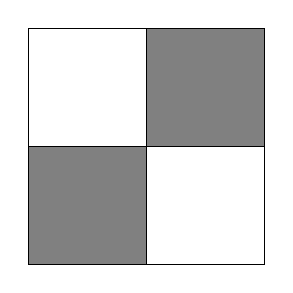
\begin{tikzpicture}	
			\draw [draw=black] (0, 0) rectangle (3, 3);
			\filldraw [draw=black,fill=gray] (0, 0) rectangle (1.5, 1.5);
			\filldraw [draw=black,fill=gray] (1.5, 1.5) rectangle (3, 3);
		\end{tikzpicture}
		\caption{Informative\\\textsc{\citeauthor{Lewis1988}-Relevant}\\ \textsc{\citeauthor{Roberts2012}-Relevant}.}\label{fig1:2-cells-relevant}
	\end{subfigure}\hfill
	\begin{subfigure}[b]{.3\linewidth}
		\centering
		\begin{tikzpicture}	
			\draw [draw=black] (0, 0) rectangle (3, 3);
			\draw [draw=black] (0, 0) rectangle (1.5, 1.5);
			\draw [draw=black] (1.5, 1.5) rectangle (3, 3);
		\end{tikzpicture}
		\caption{Informative\\\textsc{\citeauthor{Lewis1988}-Relevant}\\ \textsc{\citeauthor{Roberts2012}-Relevant}.}\label{fig1:no-cell-relevant}
	\end{subfigure}\hfill
	\begin{subfigure}[b]{.33\linewidth}
		\centering
		
\begin{tikzpicture}	
			\filldraw [draw=black,fill=gray] (0, 0) rectangle (3, 3);
			\draw [draw=black] (0, 0) rectangle (1.5, 1.5);
			\draw [draw=black] (1.5, 1.5) rectangle (3, 3);
		\end{tikzpicture}
		\caption{Uninformative\\\textsc{\citeauthor{Lewis1988}-Relevant}\\not \textsc{\citeauthor{Roberts2012}-Relevant}.}\label{fig1:all-cells-relevant}
	\end{subfigure}
\end{figure}
\begin{figure}[H]\ContinuedFloat
	\begin{subfigure}[b]{.3\linewidth}
		\centering
		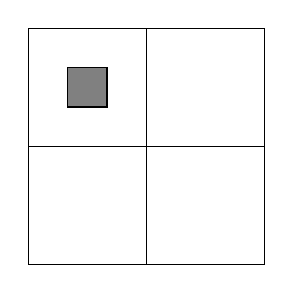
\begin{tikzpicture}	
			\draw [draw=black] (0, 0) rectangle (3, 3);
			\draw [draw=black] (0, 0) rectangle (1.5, 1.5);
			\draw [draw=black] (1.5, 1.5) rectangle (3, 3);
			\filldraw [draw=black,fill=gray] (0.5, 2) rectangle (1,2.5);
		\end{tikzpicture}
		\caption{Informative\\not \textsc{\citeauthor{Lewis1988}-Relevant}\\ \textsc{\citeauthor{Roberts2012}-Relevant}.}\label{fig1:sub-cell-relevant}
	\end{subfigure}\hfill
	\begin{subfigure}[b]{.3\linewidth}
		\centering
		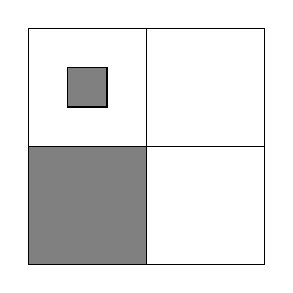
\begin{tikzpicture}	
			\draw [draw=black] (0, 0) rectangle (3, 3);
			\filldraw [draw=black,fill=gray] (0, 0) rectangle (1.5, 1.5);
			\draw [draw=black] (1.5, 1.5) rectangle (3, 3);
			\filldraw [draw=black,fill=gray] (0.5, 2) rectangle (1,2.5);
		\end{tikzpicture}
		\caption{Informative\\not \textsc{\citeauthor{Lewis1988}-Relevant}\\ \textsc{\citeauthor{Roberts2012}-Relevant}.}\label{fig1:sub-1-cell-relevant}
	\end{subfigure}\hfill
	\begin{subfigure}[b]{.33\linewidth}
		\centering
		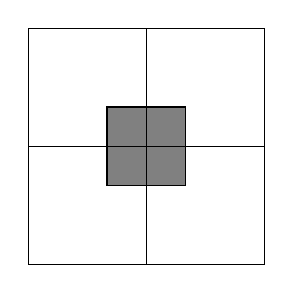
\begin{tikzpicture}	
			\filldraw [draw=black,fill=gray] (1, 1) rectangle (2,2);
			\draw [draw=black] (0, 0) rectangle (3, 3);
			\draw [draw=black] (0, 0) rectangle (1.5, 1.5);
			\draw [draw=black] (1.5, 1.5) rectangle (3, 3);
		\end{tikzpicture}
		\caption{Informative\\not \textsc{\citeauthor{Lewis1988}-Relevant}\\not \textsc{\citeauthor{Roberts2012}-Relevant}.}\label{fig1:not-relevant}
	\end{subfigure}
\end{figure}

In sum, the concept of \textsc{Relevance} (whether it follows \citeauthor{Lewis1988}'s or \citeauthor{Roberts2012}'s implementation) allows to rule-out a wide range of QuD-utterance pairs, by stating that propositions should properly relate to an existing question. We will not discuss which approach between \citeauthor{Lewis1988}'s and \citeauthor{Roberts2012}'s is best here, and will propose an incremental variant of this core concept in Chapter \ref{chap:hurford-sentences}, to deal with certain complex, out-of-the blue sentences. The next two section outline a few limitations of relevance.

\subsection{A few conceptual shortcomings of \textsc{Relevance}}

Regardless on which view of \textsc{Relevance} is adopted, relevant propositions can be added to the Common Ground, and as such, trigger an update of the CS. This, in turn, updates the QuD, which must remain a partition of the CS. It is easy to show, given how partition are ``induced'' on a set (see definition (\ref{ex1:partition-induced})), that the updated QuD on the smaller CS corresponds to the previous QuD, whose cells are pointwise intersected with the newly added proposition, and such that empty cells are filtered. This is formalized in (\ref{ex1:partitioned-context-set-update}).

\begin{exe}
	\ex{\textsc{\textbf{Updating the partitioned Context Set}}. Let $\mathcal{C}$ be a conversation, $CS(\mathcal{C})$ its Context Set, and let $Q$ be a partition of $CS(\mathcal{C})$. If a sentence $S$ denoting $p$ is uttered and relevant given $Q$ (as per (\ref{ex1:lewis-relevance}) or (\ref{ex1:roberts-relevance})), then a new Context Set $CS'(\mathcal{C})$ is derived by intersecting $CS(\mathcal{C})$ with $p$, and this new context set is partitioned by $Q'$, s.t.:\\
		$Q' = \lbrace c' \ | \ \exists c \in Q. \ c' = c \cap p \wedge c' \neq \emptyset\rbrace$}\label{ex1:partitioned-context-set-update}
\end{exe}

There are two shortcomings to the current framework. First, adding a proposition to  the CG ``mechanically'' leads to an update of the CS and of the QuD, but does not directly affect the \textit{structure} of this QuD: even if some cells should shrink, the \textit{limits} of each cell remain the same. This goes against the intuition that sometimes, sentences give rise to brand new QuDs, as exemplified by the exchange in (\ref{ex1:followup-qud}).

\begin{exe}
	\ex {--Is it raining?\\
	--Yes, I think so. I just so Ed come in with this very pretty umbrella.\\
	(Likely follow-up: Where did Ed find this umbrella?)}\label{ex1:followup-qud}
\end{exe}


Second, and relatedly, one can wonder what is supposed to happen in the case of out-of-the-blue sentences, i.e. sentences for which there is no explicit QuD. In such cases, it is generally assumed that a reasonable QuD is somehow inferred. But, given the fact that a QuD is merely a partition of the current CS, there exists many options. This dissertation will focus on how exactly QuDs are inferred, what additional constraints hold between an assertion and a QuD, and what the consequences are for pragmatic theory.

%\subsection{Relevance and the packaging of information}
%We start by showing that the felicity of disjunctions and conditionals is sensitive to \textit{overt} QuDs -- but in different ways. We take this as evidence that out-of-the-blue disjunctions and conditionals accommodate different kinds of implicit QuDs.\\
%
%If a context contrasting \textit{Paris} and \textit{France but not Paris} is set as in (\ref{ex1:qud-setting}), (\ref{ex1:hc-ns-w}) and (\ref{ex1:ldhc-ns-w}) improve (see \cite{Haslinger2023} for similar effects on disjunctions and conjunctions). This is strange: even if the context and question made \textit{Paris} (but no other French city) a relevant alternative to \textit{France}, \textit{exh} would remain IW in the consequent of (\ref{ex1:hc-ns-w}): \textit{if Jo did not grow up in Paris, she grew up in France but not Paris}, is equivalent to \textit{if Jo did not grow up in Paris, she grew up in France}. In other words, \textit{exh} (as constrained by IW) cannot leverage the contextually provided alternatives to make (\ref{ex1:hc-ns-w}) escape SR in (\ref{ex1:qud-setting}). The same applies to (\ref{ex1:ldhc-ns-w}).
%
%
%\begin{exe}
%	\ex{\textit{Context: French accents vary across countries and between Paris the rest of France.}\\
%		Al: I'm wondering where Jo learned French.\\
%		Lu: I'm not completely sure but... (\ref{ex1:hc-ns-w}) \cmark (\ref{ex1:ldhc-ns-w}) \cmark}\label{ex1:qud-setting}
%\end{exe}
%
%
%This suggests that a purely LF-based view of redundancy such as SR, may be insufficient to capture the interaction between HCs and how their context of utterance packages information. Rather, it seems that the context of (\ref{ex1:qud-setting}) makes a specific partition of the CS salient, and that this partition can be used to make otherwise infelicitous assertions accommodate a different question than the one they would evoke out-of-the-blue.
%
%Additionally, conditionals and disjunctions seem to accommodate distinct QuDs. To show this, we use the construction \textit{depending on Q, p} (\cite{Karttunen1977,Kaufmann2016}), where \textit{Q} is a question and \textit{p} a proposition. This construction has been argued to force the partition conveyed by Q to match specific live issues raised by $p$. We understand such ``live issues'' as the maximal true answers of the QuD evoked by $p$. The contrast between (\ref{ex1:depending-on-or}) and (\ref{ex1:depending-on-if}) then suggests that the \textit{France} and \textit{Belgium} answers can be matched against \textit{Q} in the disjunctive, but not in the conditional case. This in turn means that a disjunction introduces a QuD making both disjuncts maximal true answers, while a conditional does not do the same with its consequent and the negation of its antecedent.
%
%\begin{exe}
%	\ex\label{ex1:depending-on} Depending on $[$how her accent sounds like$]_{Q}$...
%	\begin{xlist}
%		\ex {Jo grew up in France \textbf{or} in Belgium. \hfill \p{}$\vee$\q }\label{ex1:depending-on-or}
%		\ex[??]{\textbf{if} Jo didn't grow up in France she grew up in Belgium. \hfill $\neg$\p{}$\rightarrow$\q} \label{ex1:depending-on-if}
%		\ex[?] {\textbf{if} Jo didn't grow up in France, she grew up in Belgium \textbf{or} in Québec. \hfill $\neg$\p{}$\rightarrow$(\q$\vee$\r)}\label{ex1:depending-on-if-or}
%		\ex [??]{\textbf{if} Jo didn't grow up in France \textbf{or} Belgium, she grew up in Québec. \hfill $\neg$(\p$\vee$\q)$\rightarrow$\r}\label{ex1:depending-on-or-if}
%	\end{xlist}
%\end{exe}
%
%
%The existence of an improvement between (\ref{ex1:depending-on-if}) and (\ref{ex1:depending-on-if-or}), and the absence of a similar improvement in between (\ref{ex1:depending-on-if}) and (\ref{ex1:depending-on-or-if}), also implies that the answers targeted by \textit{depending on Q}, when \textit{p} is conditional, are the ones made available by the consequent of \textit{p} (which is appropriately disjunctive in (\ref{ex1:depending-on-if-or}), but not (\ref{ex1:depending-on-or-if})).
%
%
%More generally, this predicts ``connectivity effects'' in disjunctions-of-conditionals, in that the antecedents and consequents respectively have to address similar QuDs; and no such effect in conditionals-of-disjunctions, in that disjuncts coming from the antecedent and consequent may be inquisitively unrelated.


\section{Conclusion and roadmap of the dissertation}

In this Chapter, we have introduced the dominant view of the semantics of questions and assertions, and of their interplay. In particular, we have seen that assertions should better be informative and relevant to the QuD raised by the conversation. In the rest of this dissertation, we will show that the interplay between questions and assertions may have implications beyond \textsc{Relevance}, and as such explain more cases of oddness that previously assumed. Specifically, we will claim that instead of being a ``good'' answer to \textit{some} QuD, an out-of-the-blue sentence must be a good answer to a \textit{good} QuD, following insights by \textcite{Katzir2015}.

Chapter \ref{chap:accommodating-quds} will continue the discussion on the pragmatics of questions, and argue that ``good'' implicit QuDs are determined from the shape of the assertive sentence itself. This is pushing the idea that assertions evoke alternatives one step further, in the sense that sentences will be taken to evoke questions (themselves derived from alternatives). These implicit questions will have a structure that consists in a generalization of the partition structure, namely, they will take the form of nested partitions of the CS.\\

In Chapters \ref{chap:redundancy}, we will claim that the process deriving questions from assertions as defined in Chapter \ref{chap:accommodating-quds}, is subject to constraints that go beyond \textsc{Relevance}, in particular \textsc{Redundancy}. A new concept of \textsc{Redundancy} will be used to explain when, and how, structurally and logically similar sentences involving disjunctions and conditionals, display distinct oddness/felicity profiles. More broadly, the introduction of constraints on QuD derivation will make way for a ``lifted'' view of pragmatic oddness, under which an assertion is not odd \textit{per se}, but rather, is odd due to its interaction with the QuDs it evokes.\\

Chapter \ref{chap:hurford-disj} will further generalize the view of \textsc{Redundancy} introduced in \ref{chap:redundancy}, in order to cover a wider variety of disjunctive sentences related to Hurford Disjunctions \parencite{Hurford1974}.\\

Chapter \ref{chap:hurford-sentences} will turn to conditional variants of Hurford Disjunctions \parencite{Mandelkern2018}, and introduce a second constraint on QuD derivation, drawing from \textsc{\citeauthor{Lewis1988}'s} and \textsc{\citeauthor{Roberts2012}'s Relevance}.\\

Lastly, Chapter \ref{chap:scalarity} will explore Hurford Disjunctions involving logically entailing scalar items, showing experimental evidence supporting the existence of a pragmatic contrast between the two possible orderings of these disjunctions. The contrast will then be explained by appealing to (incrementally) derived implicit questions, and independently motivated principles constraining question answering. 





%
%
%idea that questions and quds are diff
%questions may not denote partitions (evidence from embedding, with surprise, surprise whi not p diff from surprise who p)
%qud are partitions
%
%null hypothesis: the qud is contextually provided, it's always "out there", or, there is an overt question and the sentence gets matched against it.
%
%we explore an alternative (from katzir and singh): we have this idea qs and sentences are linked, but we dont force everything to be in the semantics
% rather, sentences have to obey constraints, that are also influences by the qs the sentnece gives rise to
% 



\section{Appendix: computing questions from propositions}\label{sec:q-derivation}

So far, we have described what could be a reasonable model for questions, in the form of partitions of the CS. But this was done without explaining how exactly such partitions are derived from the Logical Form of questions. This sketches how this is done, while further clarifying the distinction between propositions, alternatives, and questions. We will show that questions are standardly derived from closely related propositions, by abstracting over specific variables.

We will use the question \textit{In which country did Jo grow up?} as an example. The LF associated with this question is given in Figure \ref{fig1:question-lf}.

\begin{figure}[H]
	\centering
	\begin{forest}
		[\fbox{5}[$\lambda_1$][\fbox{4}[{(In which country)$_2$}] [\fbox{3}[$\lambda_2$] [\fbox{2}[[?][$t_1$]] [{\fbox{1}}[Jo][[grew up][$t_2$]]]]]]]
	\end{forest}
	\caption{LF of the question \textit{In which country did Jo grow up?}}\label{fig1:question-lf}
\end{figure}

This question involves a \textit{wh}-phrase (\textit{in which country}), which syntactically originates in an adjunct of \textit{grow up}. It is assumed that the \textit{wh}-phrase leaves a trace $t_2$ in this position. The semantics assigned to the \textit{wh}-phrase is existential, and akin to \textit{some country}. Specifically, \textit{in which country} takes a predicate of type $\langle \texttt{e}, \texttt{t} \rangle$ as argument, and returns the quantified statement that \textit{some country} verifies the predicate.

\begin{exe}
	\ex {$\llbracket$In which country$\rrbracket^w$ = $\lambda P. \ \exists l. \ l \text{ is a country in } w \wedge P(l) = 1$}
\end{exe}

The \textit{wh}-phrase outscopes another ``proto-question'' operator \parencite{Karttunen1977}. This operator takes two propositions (here, the trace $t_1$ and the proposition that \textit{Jo grew up in $t_2$}), and simply equates them. 

\begin{exe}
	\ex {$\llbracket$?$\rrbracket^w$ = $\lambda p. \ \lambda q. \ p = q$}
\end{exe}

Applying this operator successively to $t_1$ and the intension of \fbox{1}, yields the following.

\begin{exe}
	\ex {\fbox{1} = $\llbracket$Jo grew up $t_2$$\rrbracket^w = 1 \text{ iff Jo grew up in $t_2$ in $w$}$}
	\ex {\fbox{2} = $\llbracket$? $t_1$ Jo grew up $t_2$$\rrbracket^w = 1 \text{ iff } t_1 = \lambda w'. \text{ Jo grew up in $t_2$ in $w'$}$}
\end{exe}

Abstraction then applies to \fbox{2}, binds $t_2$ and yields a predicate that can then serve as an argument of the \textit{wh}-phrase. The \textit{wh}-phrase then turns this predicate into an existentially quantified expression targeting the element being questioned (here, a country).

\begin{exe}
	\ex {\fbox{3} = $\llbracket$ $\lambda_2$ ? $t_1$ Jo grew up $t_2$$\rrbracket^w = \lambda l. \ t_1 = \lambda w'. \text{ Jo grew up in $l$ in $w'$}$}
	\ex {\fbox{4} = $\llbracket$ In which country ... Jo grew up $t_2$$\rrbracket^w$\\
		\phantom{\fbox{4}}	= $\exists l. \ \text{$l$ is a country in $w$} \wedge t_1 = \lambda w'. \text{ Jo grew up in $l$ in $w'$}$}
\end{exe}

Lastly, a $t_1$ gets bound to produce a set of propositions, namely, the set of propositions that coincide with the proposition that \textit{Jo grew up in l}, for some country $l$. 

\begin{exe}
	\ex {\fbox{5} = $\llbracket$ $\lambda_1$ In which country ... Jo grew up $t_2$$\rrbracket^w$\\
		\phantom{\fbox{5}}	= $\lambda p. \ \exists l. \ \text{$l$ is a country in $w$} \wedge p = \lambda w'. \text{ Jo grew up in $l$ in $w'$}$\\
		\phantom{\fbox{5}} $\simeq$ $\lbrace p \ | \ \exists l. \ \text{$l$ is a country in $w$} \wedge p = \lambda w'. \text{ Jo grew up in $l$ in $w'$}\rbrace$
	}
\end{exe}

This example showed that the semantics of a question is derived from that of its ``assertive counterpart'', where the \textit{wh}-phrase is replaced by a quantified variable. Combined with the proto-question operator and $\lambda$-abstraction, this allows to generate a set of propositions, which only vary in terms of the variable being questioned. This set of propositions (alternatives) can then be used to induce a partition of the CS, as per (\ref{ex1:partition-induced}).


%It is also worth mentioning that under this line of analysis, questions can be properly embedded. (\ref{ex1:q-embedding}) for instance, NEED DAYAL??
%
%\begin{exe}
%	\ex {Al knows in which country Jo grew up.}\label{ex1:q-embedding}
%\end{exe}


%It is worth noting that the semantic computation laid out here, is very close in effect to how focus alternatives to an assertion are computed \cite{Rooth1992}.













